\section{Compact symmetric objects}
\begin{enumerate}
    \item Introduction to CSOs
    \item What is a CSO
    \item more on the structure of CSOs
    \item The different types of CSOs
    \item The prevalence of CSOs 
    \item CSO as candidates for UHECRs and neutrinos
    \begin{enumerate}
        
       
        \item Hillas criterion, Flux of X-ray compared to diffuse flux of UHECRs and neutrinos 
        \item Kinetic jet power
        \item Timescale analysis
    \end{enumerate}
\end{enumerate}

\subsection*{Introduction to CSOs}
In regards to other types of AGN CSO or Compact symmetric objects are similar to Seyfert Galaxies. They are characterized by their small projected size 
which in \cite{kiehlmann2023compact} is described by being less than one kiloparsec and having symmetric radio emissions on both sides of the central activity. They are also in the group
of Jetted AGN, but are distinguish from other sources of jetted AGN because the jet is non-relativistic, and there is a lack of relativistic boosting. In the paper and subsequent 
papers by \cite{kiehlmann2023compact} and their group there were some overlap in classification of some sources, were some sources were classified as CSOs when in relaity they were not. 
This was due to the fact that one overlooked two "new" properties of AGN that will also be important in this paper. CSOs are also characterized by low variability in radio and low 
apparent speed along the jet. 

\subsection{Structure of CSOs}
This section will try to constate the structure of CSOs. 



\subsection{Timescale analysis of CSOs}
In this section one will investigate the relevant timescales of a CSO and understand which processes are dominant and to the maximum energy one could expect of an escaping proton. 
First we being by determining the acceleration timescale of a proton undergoing second order fermi acceleration. The acceleration timescale is given by the equation
\begin{equation}
    t_{acc} =  \frac{\eta \epsilon}{Z e B c}
\end{equation}
where $\eta$ is the efficiency of the acceleration process with the most efficient acceleration harbouring the value $\eta \approx (1-10)$, $\epsilon$ is the energy of the particle, $Z$ is the charge of the particle, $e$ is the elementary charge, $B$ is the magnetic field strength and $c$ is the speed of light.
The value used for the magnetic field strength is $B = 10^{-2}$ G, which is the value found in \cite{bronzini2024investigating} based on the equipartition argument in the radio lobes. This value would need to change 
if investigating different regions, but in this analysis one has most data on the radio lobes. 
The value of $\eta$ is taken to be 1, which is the most efficient acceleration process.

The promesing feature for CSOs is the low variablilty. In most studies one uses the variability to determine the size of the emission region. In the case of CSOs one can use the size of the radio lobes to determine the size of the emission region or the 
estiamtes variablilty of the source which according to \cite{kiehlmann2023compact} is on the order of years to decades. This gives us an emission region of $R \sim 10^{18}$ cm.

The next timescale that is still quite trivial to introduce is the synchrotron cooling timescale. This is given by the equation
\begin{equation}
    t_{sync} = \frac{6\pi m_p^4 c^3}{\sigma_T m_e^2 B^2 E}
\end{equation}

where $m_p$ is the proton mass, $m_e$ is the electron mass, $\sigma_T$ is the Thompson cross section, $B$ is the magnetic field strength, $E$ is the energy of the particle and $c$ is the speed of light. To be precise 
this is the synchrotron loss timescale for protons and not electrons. 

The last timescale used in this analysis is the pion production timescale. This is the timescale for a proton to interact with a photon and produce a pion. This equation is more convoluted than 
the previous ones since one needs to include the relevant photon fields the proton might experience. The equation is given by
\begin{equation}
    t_{pr}^{-1}(\varepsilon_p) = \frac{c}{2\gamma_p^2} \int_{\varepsilon_{th}}^{\infty} d\varepsilon \sigma_{pr}(\varepsilon) k_p(\varepsilon) \int_{\varepsilon/2\gamma_p}^{\infty} d\varepsilon' \varepsilon'^{-2} \frac{dn}{d\varepsilon'}
\end{equation}
where $\varepsilon_p$ is the energy of the proton, $\gamma_p$ is the lorentz factor of the proton, $\varepsilon_{th}$ is the threshold energy for the interaction, $\sigma_{pr}$ is the cross section for the interaction, $k_p$ is the photon field, and $dn/d\varepsilon$ is the differential photon density.

\subsubsection{photon fields}
In order to determine the photon fields we follow \cite{Ghisellini_2009} which describe the photon fields surrounding a Blazar. The photon fields sperates into different contribution from the different regions of a classic AGN as discussed in section ... 
The different regions are the accretion disk, the broad line region, the torus and the x-ray corona. 


\textbf{Accretion disk:} The photon field emerging from an accretion disk if calculated by assuming a black body spectrum at each ring of an Shakura-Sunyaev disk and summing up its contributions. The temperature of 
each ring in the disk is given by 

\begin{equation}
    T(R) = \left(\frac{3 R_{S} L_{d}}{16 \pi R^3 \eta \sigma_{\mathrm{SB}}} \left(1-\left(\frac{3 R_{S}}{R}\right)^{\frac{1}{2}}\right) \right)^{\frac{1}{4}}
\end{equation}

Each ring of the accretion disk is assumed to be at the same temperature and emitting as a black-body spectrum. By using this temperature one can use the black body spectrum of an object with temperature T to find the intensity:

\begin{equation}
    \label{eq:BB}
    I(\nu) = \frac{2 h \nu^3}{c^2} \left(\frac{1}{\exp\left(\frac{h \nu}{k_B T}\right) - 1}\right)
\end{equation}

By integrating the intesity over all annuli of the disk one can find the total flux of the disk and from there the total energy density of the disk per frequency.
This then needs to be scaled to incorporate the location of our emitting region which sits at a distance $R$ from the accretion disk. 

The resulting spectral energy density is then given by

\begin{equation}
    U_d(\nu) = \frac{2\pi}{c} \int_{\mu_d}^1 I(\nu) d\mu
\end{equation}
where $\mu_d$ is the cosine of the angle between the location on the disk and the normal of the disk with respect to and observer.



\textbf{X-ray corona:} The photon field from the x-ray corona is assumed to be a power law spectrum with a cut off at high energies. Its total energy emitted is related to the disk Luminosity 
by the equation $L_{cor} = f L_d$ where $f$ is the fraction of the disk luminosity that is emitted by the corona. The spectral energy density of the corona is then given by 

\begin{equation}
    U_{cor}(\nu) = D(R)\left(\frac{\nu}{\nu_0}\right)^{-\alpha} \exp\left(-\frac{\nu}{\nu_{cut}}\right)
\end{equation}

The factor $D(R)$ is a scaling factor that incorporates the position of the observer in similar fashion to the disk. The integral of the spectral energy density over all frequencies should equate to the total energy density in x-ray at the location of the emitting region.

The energy density of x-ray around the central engine is given by a 

\begin{equation}
    \text{UX}(R) = \frac{f_{X} L_{d} \Gamma^2}{\pi (R_{X})^2 c} \left(1 - \mu_{X} - \beta(1 - \mu_{X}^2) + \frac{\beta^2 (1 - \mu_{X}^3)}{3}\right)
\end{equation}
where
\[
\mu_{X} = \left(1 + \frac{R_{X}^2}{R^2}\right)^{-0.5}.
\]

Here $f_{X}$ is the fraction of the disk luminosity that is emitted by the x-ray corona, $L_{d}$ is the disk luminosity, $\Gamma$ is the lorentz factor of the jet, $R_{X}$ is the size of the x-ray corona, $c$ is the speed of light, $\beta$ is the velocity of the observer in units of the speed of light.
In short the x-ray energy density stays constant until the observer is further away where it will decrease as $1/R^2$ which is to be expected.



\textbf{Broad line region:} The broad band field is assumed to be emitting a black body spectrum as in \ref*{eq:BB} which peaks at the Lyman-alpha line. The Lyman-alpha line is a spectral line of hydrogen  when the atomic electron transitions from the $n=2$ to the $n=1$ orbital corresponding to a frequency of $\nu_{\alpha} = 2.47 \times 10^{15}$ Hz. 
Similarly to the x-ray corona the spectral energy density is scaled to the region of interest and the total energy density is given by: 


\begin{equation}
    \label{eq:UBLR}
    \text{UBLR}(R) = 
    \begin{cases}
    \frac{f_{\text{BLR}} L_{d} \Gamma^2}{\pi R_{\text{BLR}}^2 c} & \text{if } R \leq R_{\text{BLR}}, \\
    \frac{f_{\text{BLR}} L_{d} \Gamma^2}{\pi R_{\text{BLR}}^2 c \beta 3} \left[2 (1 - \beta \mu_{\text{IR1}})^3 - (1 - \beta \mu_{\text{IR2}})^3 - (1 - \beta)^3\right] & \text{if } R \geq 3R_{\text{BLR}}, \\
    a R^b & \text{otherwise},
    \end{cases}  
\end{equation}
where 
\begin{align*}
    \mu_{\text{IR1}} &= \left(1 + \frac{R_{\text{BLR}}^2}{R^2}\right)^{-0.5}, \\
    \mu_{\text{IR2}} &= \left(1 - \frac{R_{\text{BLR}}^2}{R^2}\right)^{-0.5}, \\
    %b &= \log\left(\frac{\text{UBLR}(3R_{\text{BLR}}, R_{\text{BLR}}, f_{\text{BLR}}, L_{d}, \Gamma)}{\text{UBLR}(R_{\text{BLR}}, R_{\text{BLR}}, f_{\text{BLR}}, L_{d}, \Gamma)}\right) / \log(3), \\
    %a &= \frac{\text{UBLR}(R_{\text{BLR}}, R_{\text{BLR}}, f_{\text{BLR}}, L_{d}, \Gamma)}{R_{\text{BLR}}^b}.
\end{align*}


\textbf{Torus:} There is also assumed to be a dusty torus around the AGN emitting in infrared. The spectral energy density of the torus is also given by 
a black body spectrum with the temperature of the tours being set at $T_{\text{IR}} = 370$ K. The total energy density of the torus has the same relations 
as equation \ref{eq:UBLR} but with the relevant parameters for the torus.

\begin{equation}
    \text{UIR}(R) = 
    \begin{cases}
    \frac{f_{\text{IR}}L_d  \Gamma^2}{R_{\text{IR}}^2 c} & \text{if } R \leq R_{\text{IR}}, \\
    \end{cases}
\end{equation}

\subsubsection*{Total energy density}
The total energy density of the photon fields as a function of distance is then seen in figure \ref{fig:photon_fields}. 
Here one can see that the energy density of the photon fields is constant until the observer is outside the size of the respective regions. 
From the image it is clear that the biggest contributor to the total energy density becomes the IR torus, but all the regions contribute significantly to the total energy density.

\subsubsection*{Spectral energy density}
The spectral energy density of the different regions is of more interest since this is what will determine the effect of pion decay on protons accelerate in the jet or in the lobes. To create the 
SED one has estimated the dynamical scale of our system and used the total photon densities to scale the SED accordingly. The resulting SED is seen in figure \ref{fig:SED_sep}. The SED are determined also on a number of 
parameters, all which have taken from the literature. They are seen in table \ref{tab:SED_params}.

The choice of variables comes from three sources. \cite{bronzini2024investigating} and \cite{kiehlmann2023compact} which both gives the disk luminosity of CSOs sources, and which we set to $10^{43} erg/s$. \cite{Ghisellini_2009} gives the rest of parameters that relate the different regions to the disk luminosity. The biggest caveat here is that these parameters are not specific to CSOs, but to Blazars in which they are based. For the purposes of this analysis one assumes that the parameters are the same for CSOs as for Blazars, and that one would not expect any significant difference. 

\begin{table}
    \centering
    \begin{tabular}{|c|c|}
        \hline
        Parameter & Value \\
        \hline
        $L_{d}$ & $10^{43}$ erg/s \\
        $GM$ & $G 10^{8} M_{\odot}$ \\
        $RS$ & $\frac{2GM}{c^2}$ \\
        $\eta$ & 0.1 \\
        $f_{X}$ & 0.3 \\
        $R_{X}$ & 30$ RS $\\
        $\beta$ & 0.4 $c$\\
        $f_{\text{BLR}}$ & 0.1 \\
        $R_{\text{BLR}}$ & $10^{17} \sqrt{L_{d}/10^{45}}$ cm \\
        $f_{\text{IR}}$ & 0.5 \\
        $R_{\text{IR}}$ & $2.5 10^{18}\sqrt{L_{d}/10^{45}}$ cm \\
        $\Gamma$ & 1.1 \\
        \hline
    \end{tabular}
    \caption{Parameters used to determine the SED of the different regions.}
    \label{tab:SED_params}
\end{table}
\begin{figure}
    \centering
    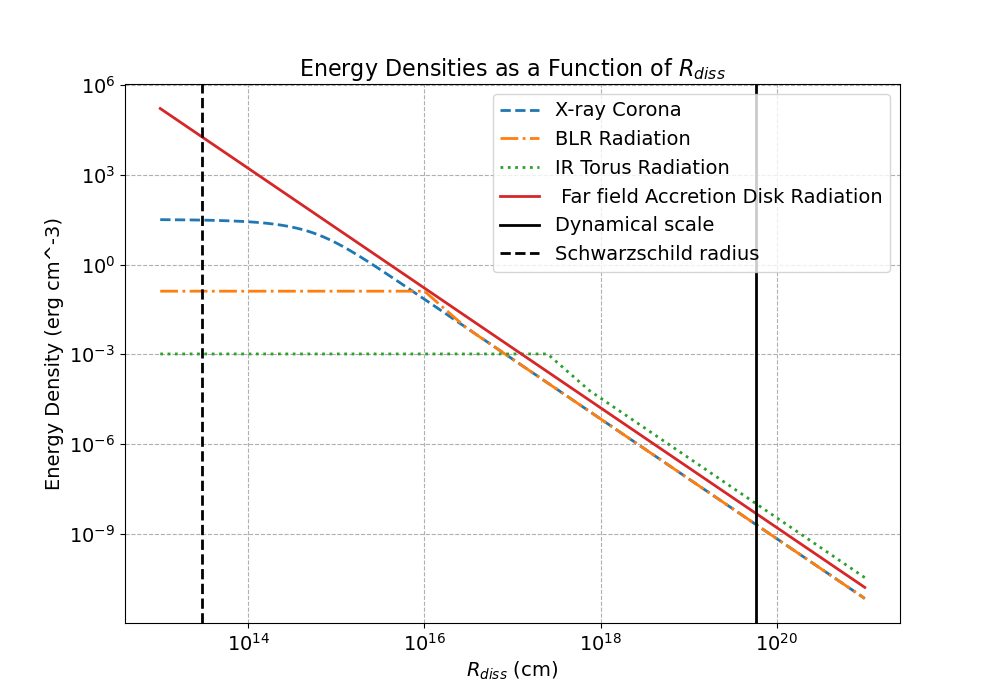
\includegraphics[width=.5\textwidth]{C:/Users/henri/OneDrive/Documents/NTNU/Semester 10/Masteroppgave/Plots/Energy_densities.png}
    \caption{The total energy density of the photon fields as a function radius from central engine.}
    \label{fig:photon_fields}
\end{figure}


\begin{figure}
    \centering
    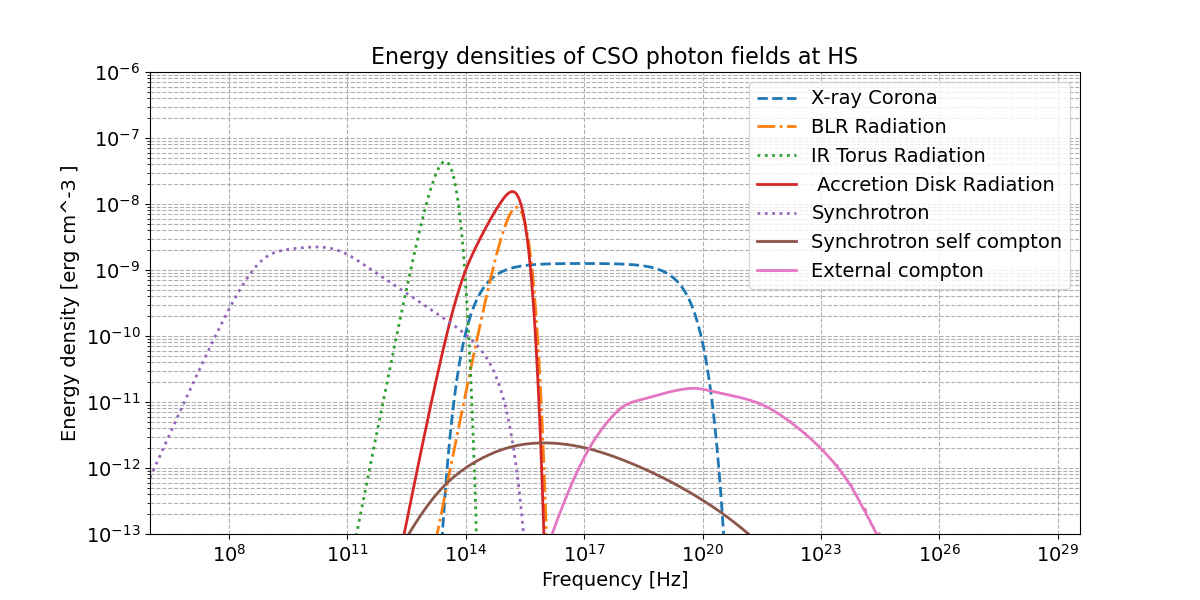
\includegraphics[width=.5\textwidth]{C:/Users/henri/OneDrive/Documents/NTNU/Semester 10/Masteroppgave/Plots/SEDs_sep.png}
    \caption{The spectral energy density at distance R}
    \label{fig:SED_sep}
\end{figure}

\begin{figure}
    \centering
    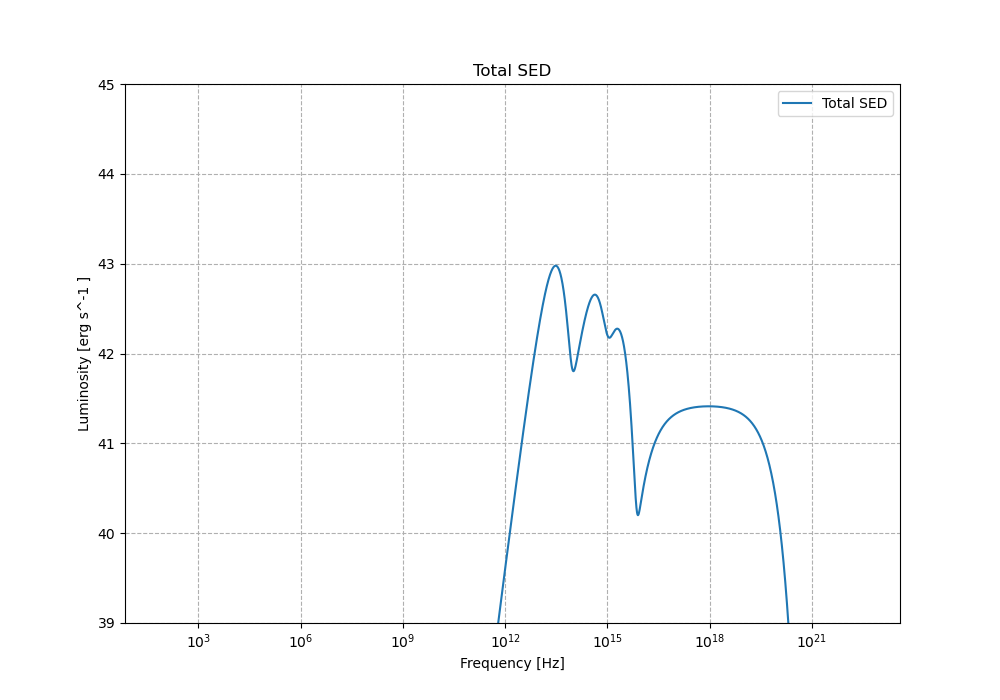
\includegraphics[width=.5\textwidth]{C:/Users/henri/OneDrive/Documents/NTNU/Semester 10/Masteroppgave/Plots/SED.png}
    \caption{Luminosity of the different components of the CSO that are close by the central engine. Missing synchrotron and IC part which is most prominent }
    \label{fig:Lum_SED}
\end{figure}

\subsection{Classification of CSO}
From the papers of \cite{kiehlmann2023compact} to \cite{readhead2023compact}, and from \cite{sullivan2024smallscale} there is a clear quite new classification of CSOs. The classification is based on firstly CSOs being edge brightened or edge dimmed. Edge brightened sources which will onwards be refered as CSO 2s are bright in radio in their lobes, and CSO 1s or edge dimmed are thought to be CSOs that have stalled. 

The big picture on CSOs is that they are a group of very short-lived sources that are ignited by transient events. Saying if the ignition of their jets are due to transient event such as tidal disruption event are covered in \cite{sullivan2024smallscale} and for the purposes of this study not necessary to discuss, but start a very interesting conversation. CSOs are then symmetric with the expansion of their jets into the interstellar medium visible from radio telescope. The symmetry of the jets is a key feature of CSOs and makes them unique in the sense of jetted-AGN since they have little to no features of relativistic beaming.   


\subsection{Catalouge of Bona fide CSO}
In order to study these sources there will always be a need for observational data. This fact combined with the fact that CSOs are a somewhat new class of AGN mean that there are no large catalogues of pure CSOs, and that many other catalogues misnomer sources as CSOs. This chapter will rely heavilly on \cite{kiehlmann2023compact} in which this is discussed and where they define a bona fide catalogue of 79 CSOs. The catalogue will allow us as it has in this paper to say more concrete infromation about the sources we are studying.



\subsection{Prevalence of CSOs}







\subsection{Stability in jet expansion and lobes.} The most promesing feature of CSOs which we will see as a key feature in the section on time-scales is the stability of the lobes in radio emission, the stability of the jet expansion and the stability of most wavelengths in emissions. In \cite{bronzini2024investigating} they report no significant variablilty of one CSO source in gamma rays, variability of the order of years in x-ray, with the broadband SED showing variability on the timescales of years. This is a clear distincsion from other jetted AGN which are known to be highly variable. Having stable systems allows for more efficient acceleration of ions, and significantly increases the possibility of producing UHECRs. 